\section{Model verification}\label{sec:verification}

To ensure that our implementation does not contains bug and correctly implements
the model we have performed various tests:
\begin{description}
	\item[Memory Check] We have used Valgrind on all tests defined in
		\code{tests.ini} to verify that there were no bad memory
		accesses and memory leaks.
	\item[Graphical Test] We have run the ``Simple'' configuration in the
		\omnetpp{} QT environment to check visually that the network
		works as expected. We have also collected statistics for these
		runs and checked that they are consistent with what we have seen
		in the graphical environment. This test has been also performed
		for the ``DocExample'' configuration, as shown in
		\figref{fig:snapshot}.
	\item[Step-by-Step Debug] We have also debugged the ``Simple''
		configuration step-by-step to check that our code takes the
		expected code path.
	\item[Event Trace Check] For the ``Simple'' configuration we have also
		logged and verified the event trace in order to ensure that
		events are scheduled in the correct order.  \item[Deterministic
		Test] We have run the ``Deterministic'' configuration in
		multiple repetitions and verified that the results were the same
		for all runs\footnote{File
		\code{analysis/DeterministicTest/zero-variance-test.ipynb}
		contains the full analysis for this test. It checks that all the
		residuals for each observation are zero.}.
	\item[Degeneracy Test] We have run the ``UserDegeneracy'' configuration
		and tested that the network simply does nothing and all recorded
		statistics are equal to zero with zero users, while only a
		message is sent (not heard by anyone) with one user. We have run
		the ``NoRadius'' configuration and checked that the first user
		sending the message is not able to reach anyone. We have run the
		``Unreachable'' configuration (two users at long distance) and
		verified that the user sending out the message is not able to
		reach the other.
	\item[Continuity Test] We have run the ``Continuity'' configuration and
		verified that all the measured quantities increase as the number
		of users increases. As an example, in \figref{fig:continuity} we
		can see that the total broadcast time needed to reach the 95th
		percentile of the users, the number of collisions and the total
		number of messages sent increase with the number of users in the
		network\footnote{File
		\code{analysis/ContinuityTest/continuity-test.ipynb} contains
		the Python script used to generate these images.}. We note that
		the test has been performed by varying the total number of user
		but keeping the user density fixed \idest{by keeping the
		\(\frac{N}{A}\) ratio fixed}.
\end{description}

\savegeometry{normal}
\clearpage
\newgeometry{margin=1pt}
\begin{figure}[p]
	\centering
	\begin{subfigure}[b]{0.45\textwidth}
		\centering
		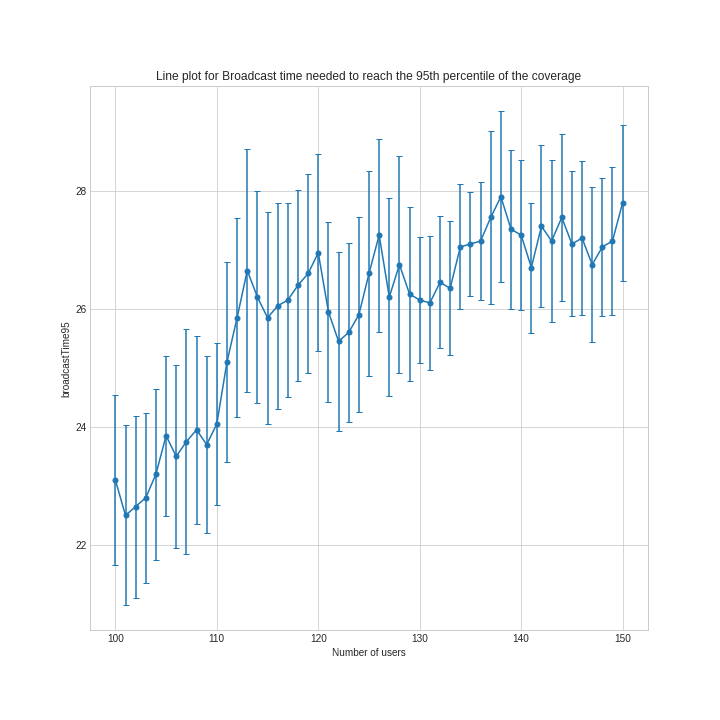
\includegraphics[width=\textwidth]{img/continuity-broadcasttime}
		\caption{Broadcast time to reach the\\95th percentile of the
		users}
	\end{subfigure}
	\hfill
	\begin{subfigure}[b]{0.45\textwidth}
		\centering
		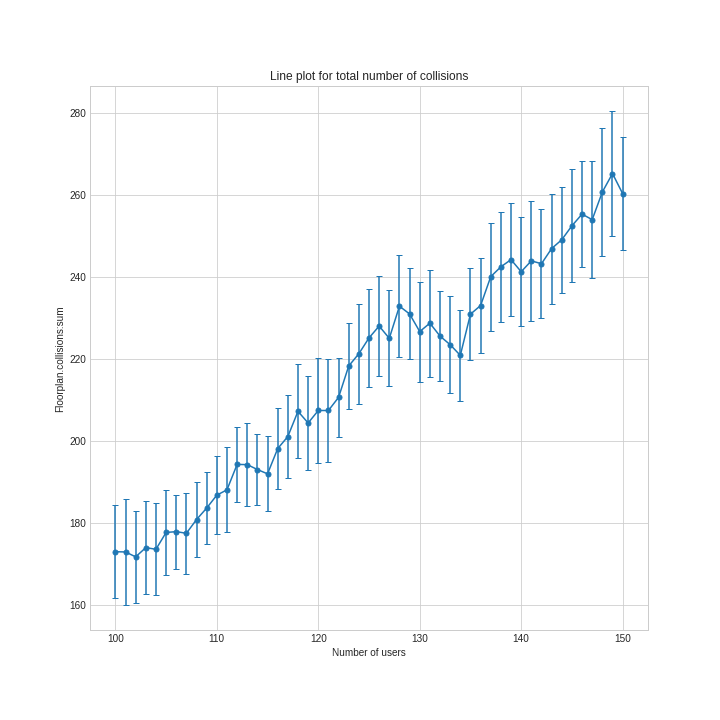
\includegraphics[width=\textwidth]{img/continuity-collisions}
		\caption{Total number of collisions}
	\end{subfigure}
	\begin{subfigure}[b]{0.35\textheight}
		\centering
		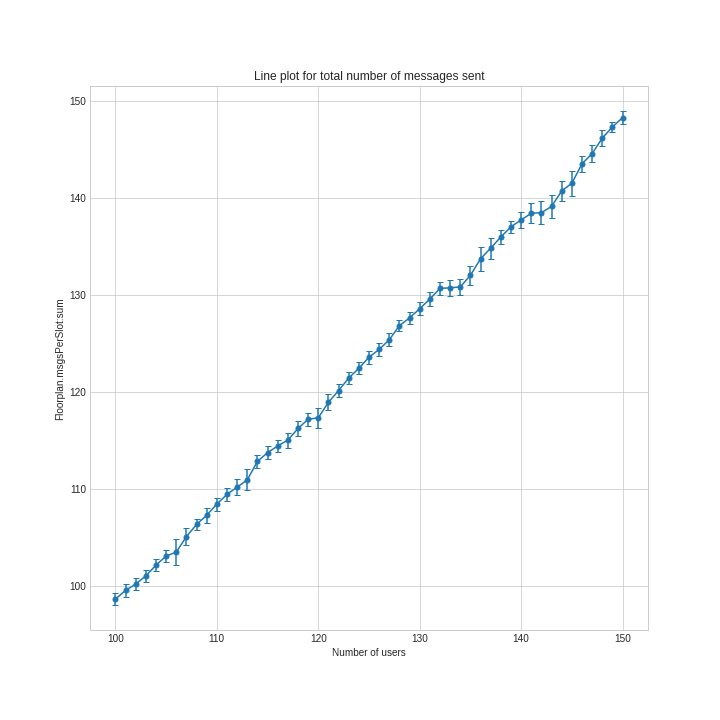
\includegraphics[width=\textwidth]{img/continuity-msgssent}
		\caption{Total number of messages sent}
	\end{subfigure}
	\caption{Continuity test (\(90\%\) confidence
	intervals)}\label{fig:continuity}
\end{figure}
\clearpage
\loadgeometry{normal}
